\chapter{Introduction} \label{chap:introduction}Economists assert manufacturing to be a wealth-producing sector of an economy, since manufacturing process involve the processes to transform raw materials into finished goods on a large scale. Manufacturing world thrives upon many complex variables. In the recent years, due to innovations in \acs{ICT} the focus of supply and demand are shifting, thus manufacturing industry is experiencing complex supply chains. Customers demanding high levels of individualized products are driving fierce competition in pricing and forcing manufacturers to strive for highest levels of efficiencies. Still manufacturers can develop effective survival strategies amidst all these turbulences \reffig{fig:1.1} if they are able to continuously adapt their organizational structures \cite{WESTKAMP}.

The challenge for adaptive manufacturing is to access all available information when it is needed, where it is needed, and in the form it is most useful to drive optimal actions and responses \refsection{IOT}. Adaptive manufacturing also enables manufacturers to generate and apply data-driven manufacturing intelligence throughout the life-cycle of design, engineering, planning and production.

A new wave of technological changes \refsection{ind4} is already driving a paradigm shift in manufacturing. Manufacturing sector is at the verge of a new industrial revolution which promises all range of opportunities for innovation in terms of smarter industrial processes, new business models and customized products. The new technological wave builds on the concept of interaction between the real and virtual worlds which becomes the core of the manufacturing processes. Both production equipment and manufactured products are now able to gather, process and analyze data of the physical world and interact with each other autonomously.
\begin{figure}[h!]
	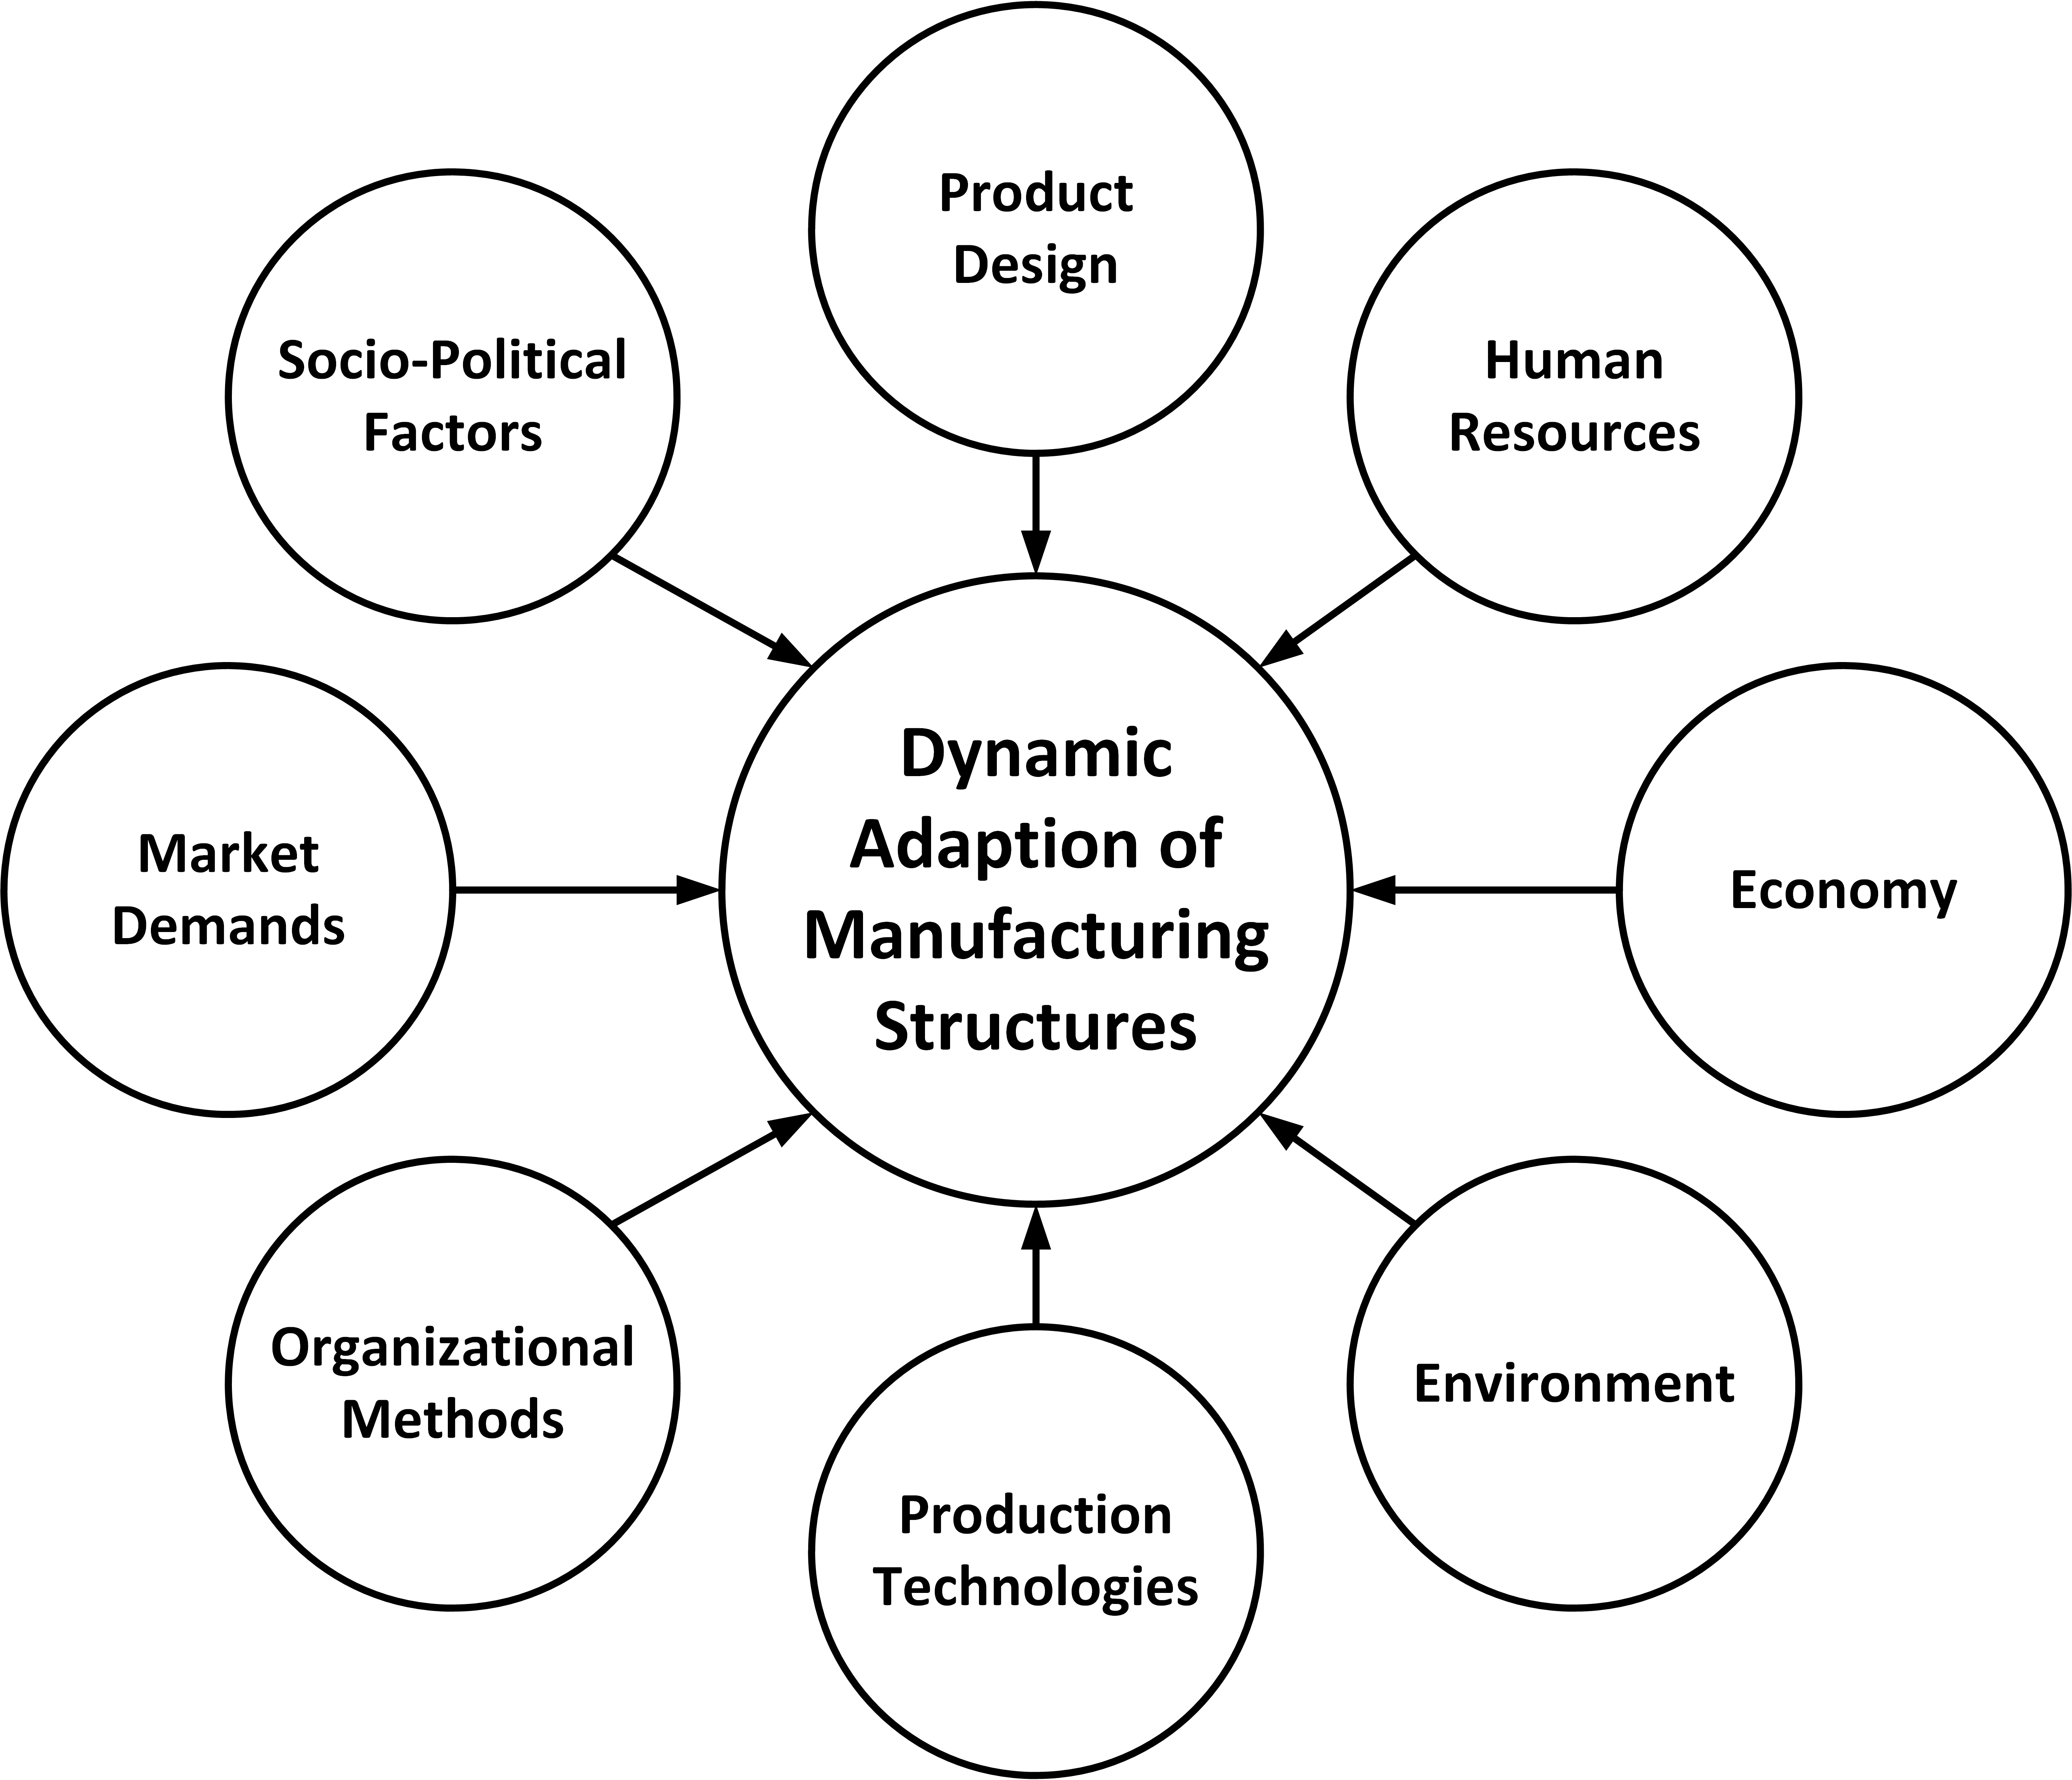
\includegraphics[scale=0.4]{./gfx/addmanustr}
	\centering
	\caption{Adapting the Structures of Manufacturing \cite{WESTKAMP}}
	\label{fig:1.1}
\end{figure}

To increase the efficiency of production process, automation, optimization, and dynamic adaption became the most important requirements in manufacturing sector. Since the dawn of sensors and networking technologies \refsection{IOT} vital information can be gathered before-hand to decide the most suitable and optimized process.  The selection of each execution step may depend on different factors as new technological advancements provide more solution options to the same kind of problems. Manually conducted assembly tasks may provide alternatives to the existing automation methods depending on the current demand, status of the machinery, and occupation of the machinery \cite{TIMURCIRP}. Situations can be observed using smart-systems \refsection{CPS} which enable the application of well-adopted business process modeling and execution  solutions in the context of manufacturing companies and tracking of activity flows in the real world \cite{CONWORKFLOW}.

Production or Manufacturing processes can be modeled using business process process modeling languages e.g. the Business Process Execution Language (\acs{BPEL}) \cite{BPELSPEC} or the Business Process Model and Notation (\acs{BPMN}) \cite{OMGSPEC}. After modeling, the process models are deployed on compliant work-flow engines for an automated execution. But these paradigms don not support adaptive and flexible execution of business processes in manufacturing sector. By not considering these adaptations, the manufacturing companies lose their revenue and edge in market by remaining reluctant to structural changes on time \cite{TIMURCIRP,CONWORKFLOW}.
\section{Problem Statement}
Manufacturing processes need to be updated regularly to stay competitive in the market was the theme of last section. With the emergence of Internet of Things \refsection{IOT}, the manufacturing processes can be made smarter to leverage the next industrial revolution - Industry 4.0 \refsection{ind4}.

Sungur et al. \cite{TIMURCIRP} presented a novel approach to support \textit{Context-sensitive Adaptive Production Process} in their research work. They extended production processes, which contain a sequence of predefined sets of sub-processes, with \textit{Context-sensitive Execution Steps (\acs{CES})} \refsection{conces}. For each \acs{CES}, context-relevant sub-processes are chosen and desired processes are elected, optimized, deployed and executed \cite{TIMURCIRP}.

\acs{CES} approach dictates a way in which processes can possibly adapt themselves to the execution context. In each context, there can be multiple alternatives for the same process goals and the best needs to be selected and executed at runtime \cite{TIMURCIRP}.
\section{Scope of Work}